\documentclass[11pt, aspectratio=169]{beamer}
%\documentclass{beamer}
\setbeamertemplate{navigation symbols}{}
\usetheme{Boadilla}
\usecolortheme{beaver}
\usepackage{caption}


\usepackage{tikz} 
\usepackage{adjustbox}

\usepackage{graphicx}
\usepackage{subcaption}
\usepackage{algorithm}
\usepackage{algpseudocode}
%\usepackage[noend]{algorithmic}
\usepackage{amsmath}
\usefonttheme{professionalfonts}
\usepackage{helvet}
\renewcommand{\familydefault}{\sfdefault}
%\renewcommand{\figurename}{Gambar}
\usepackage{hanging}
\usepackage{lipsum}
\usepackage{listings}
\newcommand\blfootnote[1]{%
  \begingroup
  \renewcommand\thefootnote{}\footnote{#1}%
  \addtocounter{footnote}{-1}%
  \endgroup
}
\setbeamertemplate{caption}{\insertcaption}

\setbeamertemplate{footnote}{\tiny \hangpara{1em}{1}\makebox[1em][l]{\insertfootnotemark}\footnotesize\insertfootnotetext\par}
\hyphenation{}

\usepackage{ragged2e}
\renewcommand\thempfootnote{\arabic{mpfootnote}}



%=======================================================
%KETERANGAN FRAME
\title[Downscaled DVB-T2 LDPC Codes]{Downscaled LDPC Codes for Indonesia Digital Video Broadcasting Terrestrial 2nd Generation (DVB-T2)}
%\subtitle{Avoiding Common Mistakes}
\author[Afa]{ \vspace{-0.1in}

\includegraphics[height=0.35in]{gambarafa/logoSOFTT}
\hspace{0.05in}

\includegraphics[height=0.35in]{gambarafa/adwitech}
\hspace{0.05in}

\includegraphics[height=0.35in]{gambarafa/telu.jpg}\\ \quad \\Citra Yasin Akbar Fadhlika and Khoirul Anwar}
\institute[AdWiTech, Telkom Univ.] { The Center for Advanced Wireless Technologies (AdWiTech), Telkom University,\\
Jl. Telekomunikasi No. 1, Terusan Buah Batu, Bandung, 40257 Indonesia.\\
E-mail: \{\textit{citrayaf@student., anwarkhoirul@\}telkomuniversity.ac.id}
\blfootnote{\tiny{This research is supported in part by the World Class Research Grant for T3LESDM-Net, 20192021.}}
}

\date[November $19^{th}, 2019$]{\small Presented at the $3^{rd}$ International Conference on 3rd SOFTT 2019\\
 Kuala Lumpur, Malaysia }


%			LET'S START YEYEYEYYEYE
%========================================================
% Let's get started the document
\begin{document}
\justifying

\begin{frame}
  \titlepage
\end{frame}
\begin{frame}{Outline}
  \tableofcontents
  % You might wish to add the option [pausesections]
\end{frame}
%-----------------------------------------------------------------------


%=======================================================
%=======================================================
\section{Motivation and Problem}
%--------------------------------------
\begin{frame}{Motivation and Problem}
%--------------------------------------
\begin{figure}
\centering

\includegraphics[scale=0.35]{gambarafa/migrasi}
\caption{Indonesia Digital Television Standard Migration.}
\label{downlink} 
\end{figure}
\vspace{-10pt}
\begin{itemize}
\justifying
\item DVB-T2 replaces DVB-T standard as the Indonesia terrestrial digital television standard.\blfootnote{\tiny{Minisitry of Communications and Informatics Indonesia Regulation Number: 05/PER/M.KOMINFO/2/2012.}}
\item Absence of the suitable LDPC codes for Indonesia channel model leading to an optimal performances.
\end{itemize}
\end{frame}

%=======================================================
%=======================================================
\section{System Model of DVB-T2}

%--------------------------


%--------------------------
\begin{frame}{System Model of DVB-T2}
%--------------------------
\vspace{-10pt}
\begin{figure}
\centering 
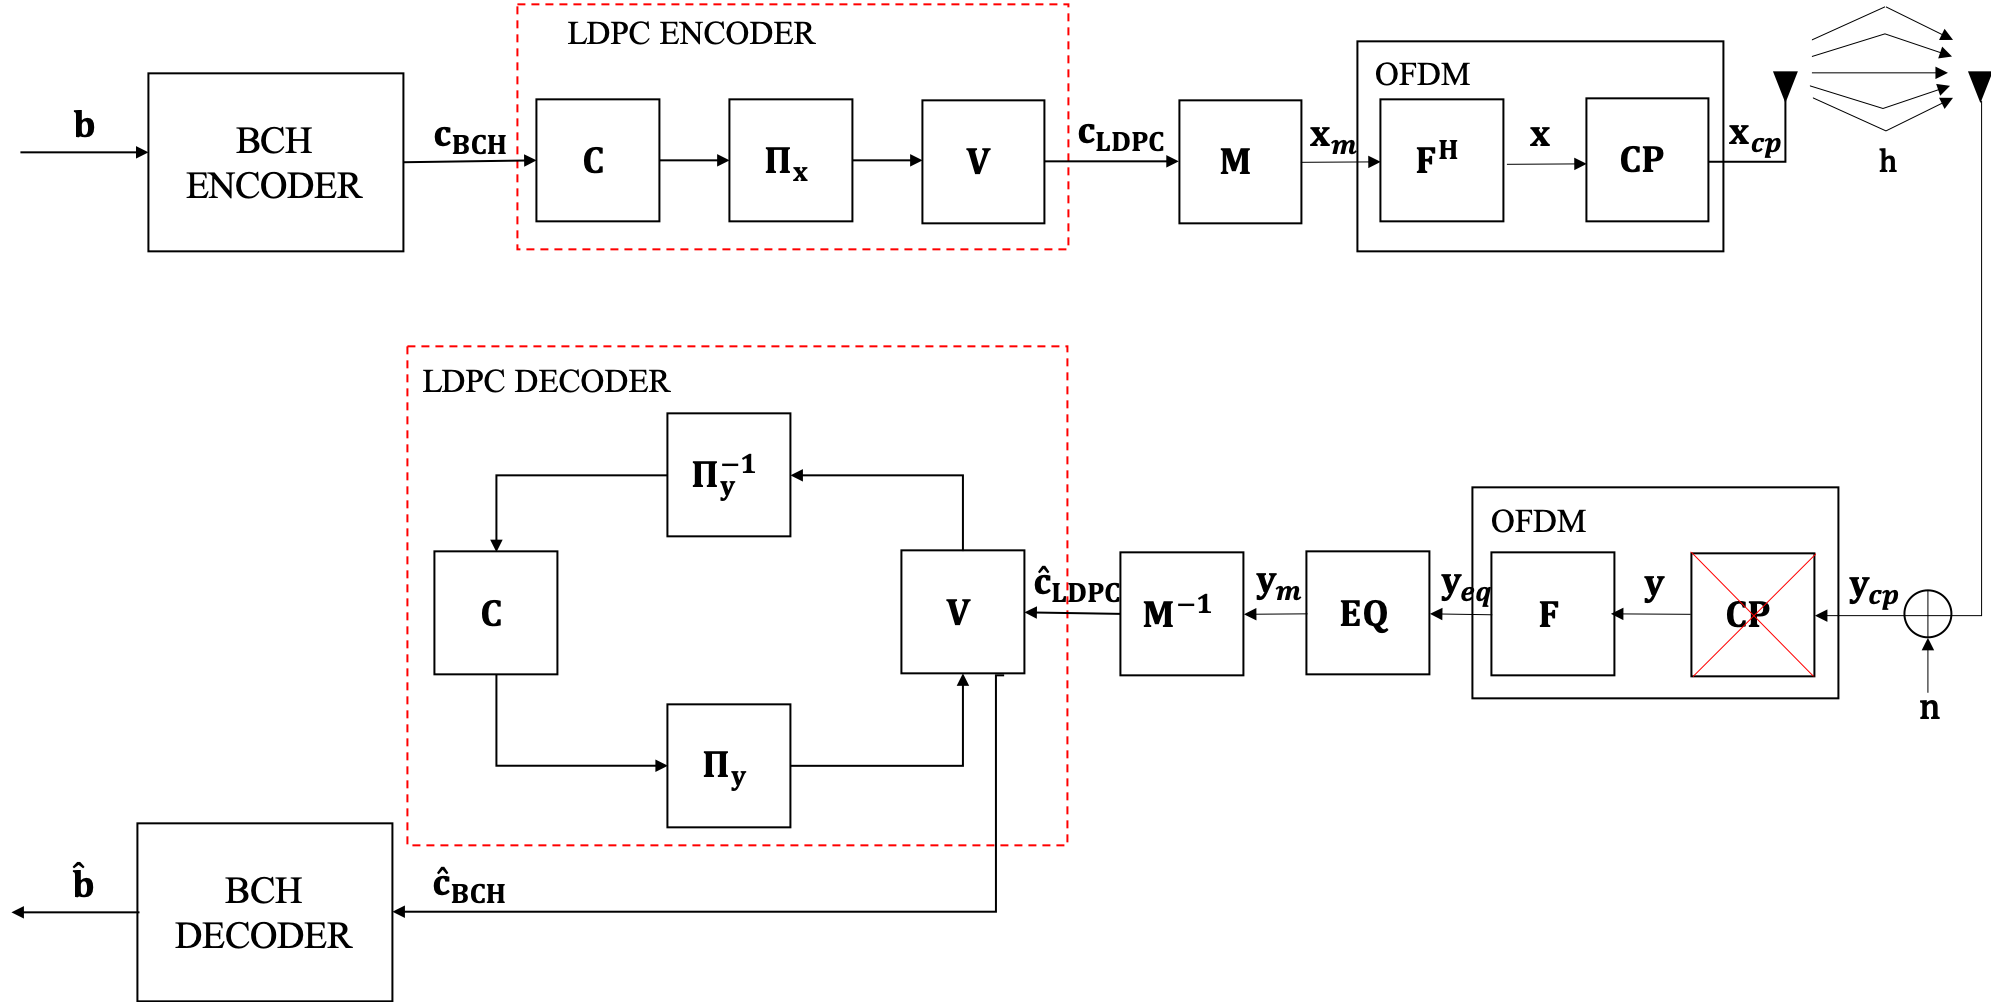
\includegraphics[scale=0.25]{gambarafa/sistemmo}
\label{sistemmodelMQCLDPC} %~\ref{kucing}
\end{figure}
\vspace{-5pt}
\begin{itemize}
\item The structure of LDPC encoder and decoder are adapted from ETSI TS 102 831 V1.2.1.
\item The modulation $\mathbf{M}$ is Quadrature Phase Shift Keying (QPSK). 
\item We consider multipath channel $\mathbf{h}$ using Bandung DVB-T2 channel model.
\end{itemize}
%\begin{columns}
%\hspace{10pt}
%\column{.4\textwidth}
%\small{$\mathbf{b}$ : information bits\\
%$\mathbf{C}$ : check nodes\\
%$\Pi$ : interleaver\\
%$\mathbf{V}$ : variable nodes\\
%$\mathbf{c_{BCH}}$ : BCH codewords\\
%$\mathbf{c_{LDPC}}$ : LDPC codewords\\
%$\mathbf{M}$ : modulator\\
%$\mathbf{x_{cp}}$ : transmit symbols\\
%}
%\column{.4\textwidth}
%\small{$\mathbf{h}$ : Bandung channel\\
%$\mathbf{n}$ : noise\\
%$\mathbf{y_{cp}}$ : received symbols\\
%$\mathbf{M^{-1}}$ : demodulator\\
%%$L_{ch}$ : LLR channel\\
%%$I_E$ : extrinsic information\\
%%$I_A$ : mutual information\\
%$\mathbf{\hat{c}_{LDPC}}$ : estimated LDPC codewords\\
%$\mathbf{\hat{c}_{BCH}}$ : estimated BCH codewords\\
%$\mathbf{\hat{b}}$ : estimated bits information\\}
%\end{columns}
\end{frame}
%=======================================================
%=======================================================
\begin{frame}{DVB-T2 LDPC Codes}
%--------------------------
\vspace{-1.75cm}
\begin{figure}
\centering 
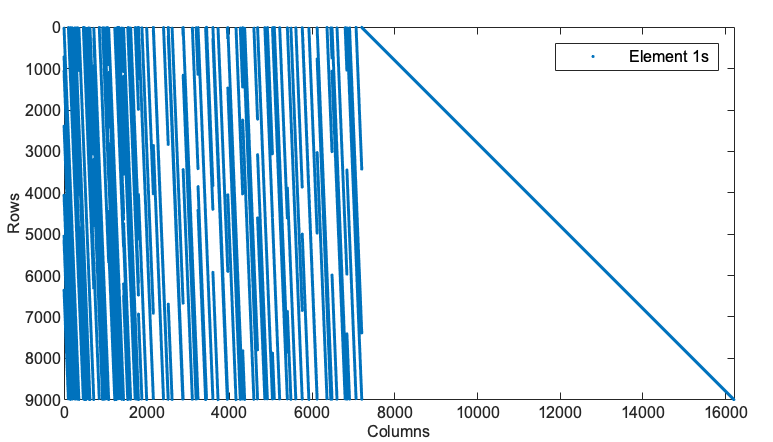
\includegraphics[scale=0.45]{gambarafa/hs(1-2)-2}
\centering 
\label{sistemmodelMQCLDPC} %~\ref{kucing}
\end{figure}

\begin{itemize}
%\item SIMPLE : Small block size less than 2000
\item DVB-T2 LDPC codes according to ETSI TS 102 831 V1.2.1 have block-length $N_{LDPC}=16200$ and $N_{LDPC}=64800$.

\item LDPC codes with $N_{LDPC}=16200$ have code rates $R=\left \{ \frac{4}{9}, \frac{3}{5}, \frac{2}{3},\frac{11}{15},\frac{7}{9},\frac{37}{45} \right \}$

\item We proposed DVB-T2 LDPC codes with $N_{LDPC}=16200$ having code rates $R=\frac{4}{9}$.
%\item The systems use narrowband system with single carrier transmission.
%\item Channels are Additive White Gaussian Noise (AWGN) and frequency-flat Rayleigh fading.
%\item Perfect channel synchronization and estimation.
%\begin{itemize}
%\item Matrix Generator $G$ in encoder.
%\item Parity Check Matrix $H$ in decoder. 
%\end{itemize}
%\vspace{-0.35cm}
%\begin{eqnarray}
%\mathbf{G}\cdot \mathbf{H}^T&=&0.
%\end{eqnarray}
\end{itemize}

\vspace{-20pt}
%\begin{figure}
%\centering 
%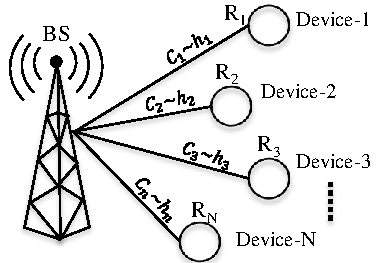
\includegraphics[scale=0.85]{pics/downlink2.pdf}
%\caption{Configuration of downlink IoT wireless communication systems.}
%\label{massiveiot} %~\ref{kucing}
%\end{figure}

\end{frame}
%%--------------------------
%\begin{frame}{Basic Theory}
%%--------------------------
%\begin{itemize}
%\item Low-Density Parity-Check (LDPC) codes were introduced by Gallager in his PhD dissertation in the 1960s.
%\item LDPC codes are binary linear block codes with a sparse parity-check matrix $\mathbf{H}$ that has most of its elements as 0s.
%%\item Low latency channel coding and low complexity.
%\end{itemize}
%\begin{columns}
%\column{.45\textwidth}
%\begin{eqnarray}
%\mathbf{G}&=&[I_k\; P],\\
%\mathbf{H}&=&[-P^T\; I_{n-k}],\\
%\mathbf{G}\cdot \mathbf{H}^T&=&0.
%\end{eqnarray}
%\column{.55\textwidth}
%\begin{figure}
%\centering %taro di tengah
%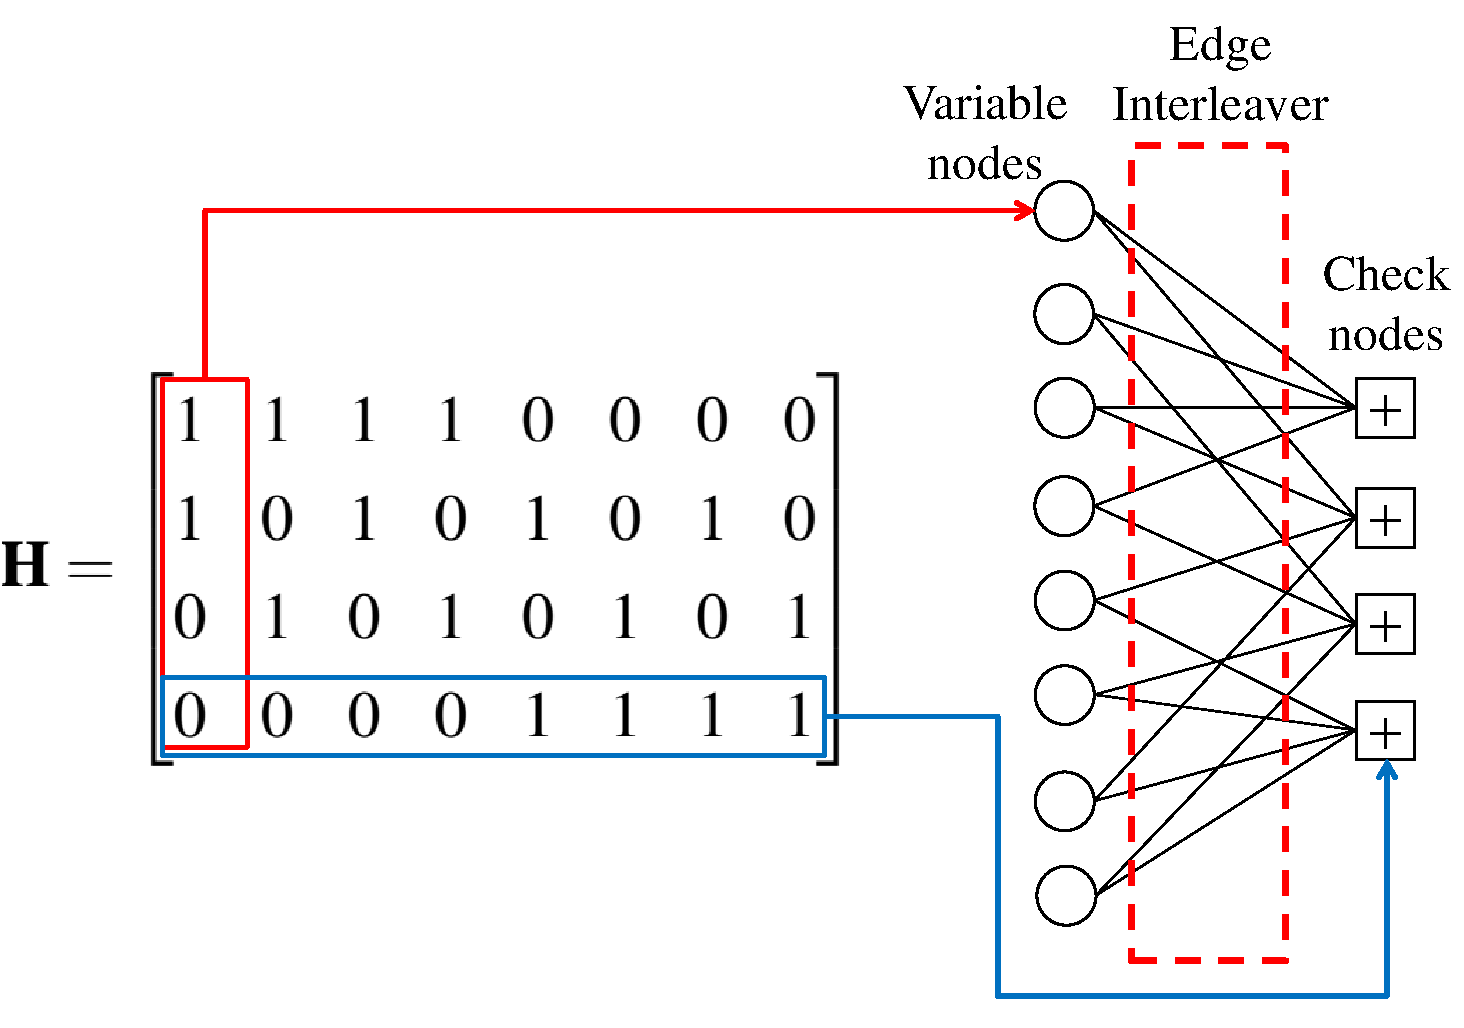
\includegraphics[scale=0.25]{pics/bipartitH1.pdf}
%\caption{Bipartite graph of parity check matrix $\mathbf{H}$.}
%\label{bipartitH} 
%\end{figure}
%\end{columns}
%\end{frame}
\begin{frame}{Tanner Graph of The Proposed DVB-T2 LDPC Codes}
%--------------------------
\vspace{-0.5cm}
	\begin{figure}
		
		\centering
		
		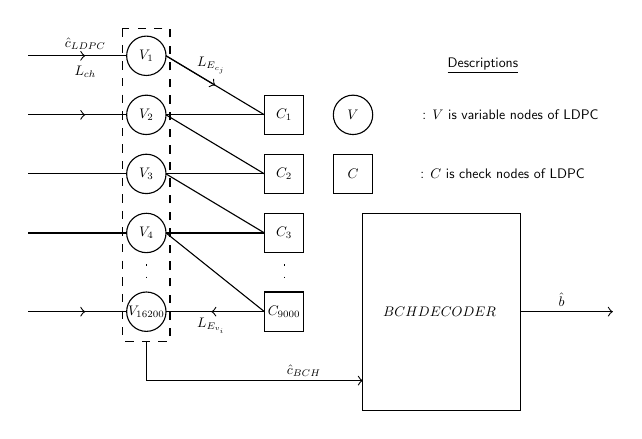
\begin{tikzpicture}[scale=0.5, transform shape]

		
		\draw (1,-6) -- (2.45,-6)[->];
		\node at (2.45,-5.7) {$\hat{c}_{LDPC}$};
		\node at (2.45,-6.4) {$L_{ch}$};

		\draw (1,-6) -- (3.5,-6);
		\draw (1,-7.5) -- (3.5,-7.5);
		\draw (1,-7.5) -- (2.45,-7.5)[->];
		\node at (5.65,-6.25) {$L_{E_{c_{j}}}$};

		\draw (1,-9) -- (3.5,-9);
		\draw (1,-10.5) -- (3.5,-10.5);
		\draw (1,-12.5) -- (3.5,-12.5);
		\draw (1,-12.5) -- (2.45,-12.5)[->];
		\node at (5.65,-12.85) {$L_{E_{v_{i}}}$};

		
		
		\draw (7,-8) rectangle (8,-7); \node at (7.5,-7.5) {$C_1$};
		\draw (7,-8.5) rectangle (8,-9.5); \node at (7.5,-9) {$C_2$};
		\draw (7,-10) rectangle (8,-11); \node at (7.5,-10.5) {$C_3$};
		\draw (7.5,-11.3) [loosely dotted]-- (7.5,-11.7);
		\draw (7,-12) rectangle (8,-13); \node at (7.5,-12.5) {$C_{9000}$};
		
		\draw (4,-6) circle [radius=0.5]; \node at (4,-6) {$V_{1}$};
		\draw (4,-7.5) circle [radius=0.5]; \node at (4,-7.5) {$V_{2}$};
		\draw (4,-9) circle [radius=0.5]; \node at (4,-9) {$V_{3}$};
		\draw (4,-10.5) circle [radius=0.5]; \node at (4,-10.5) {$V_{4}$};
		\draw (4,-11.3) [loosely dotted] -- (4,-11.7);
		\draw (4,-12.5) circle [radius=0.5]; \node at (4,-12.5) {$V_{16200}$};
		\draw (3.4,-5.3) [dashed] rectangle (4.6,-13.25);
		\draw (4,-13.25) -- (4,-14.25);
		\draw (4,-14.25) -- (9.5,-14.25) [->];
		\draw (9.5,-10)  rectangle (13.5,-15); \node at (11.45,-12.5) {$BCH DECODER$};
		\draw (13.5,-12.5) -- (15.85,-12.5) [->];\node at (14.55,-12.2) {$\hat{b}$}; 
		\node at (8,-14) {$\hat{c}_{BCH}$};

		
		\draw (4.5,-6) -- (7,-7.5);
		\draw (4.5,-6) -- (5.75,-6.75)[->];
		
		\draw (4.5,-7.5) -- (7,-7.5);
		\draw (4.5,-7.5) -- (7,-9);
		\draw (4.5,-9) -- (7,-9);
		\draw (4.5,-9) -- (7,-10.5);
		\draw (4.5,-10.5) -- (7,-10.5);
		\draw (4.5,-10.5) -- (7,-12.5);
		\draw (4.5,-12.5) -- (7,-12.5);
	
		\draw (5.65,-12.5) -- (7,-12.5)[<-];
		
	\node at (12.55,-6.25) {\underline{Descriptions}};
		\draw (9.25,-7.5) circle [radius=0.5]; \node at (9.25,-7.5) {$V$};
		\node at (13.25,-7.5)  {: $V$ is variable nodes of LDPC};

        \draw (8.75,-9.5) rectangle (9.75,-8.5); \node at (9.25,-9) {$C$};
        \node at (13.05,-9) {: $C$ is check nodes of LDPC};

        % \node at (13.55,-7.9) {: are degree distribution of EP VND};

        % \node at (13.55,-8.6) {: are degree distribution of EP CND};
		
		
		\end{tikzpicture}
		\label{fig:tg}
	\end{figure}
	\vspace{-0.45cm}
$L_{E_{v_{i}}}$ and $L_{E_{c_{j}}}$ are expressed\blfootnote{\tiny{S. ten Brink, “Convergence Behavior of Iteratively Decoded Parallel Concatenated Codes,” IEEE Transactions on Communications, vol. 49, no. 10, pp. 1727–1737, Oct 2001.}}
\begin{columns}
\column{.5\textwidth}
\vspace{-0.2cm}
\begin{equation}
L_{E_{v_{i}}}(n)=L_{ch}+\sum_{j=1,j\neq i}^{d_{v_{n}}} L_{A_{v_j}},
\end{equation}

\column{.5\textwidth}
\vspace{-0.1cm}
\begin{equation}
L_{E_{c_{j}}}(k)=\sum_{i=1,i\neq j}^{d_{c_{k}}}\boxplus L_{A_{c_{i}}}.
\end{equation}


\end{columns}

\end{frame}


%--------------------------
\begin{frame}{The Proposed Parity Check Matrices }
%--------------------------
\vspace{-0.5cm}
\begin{table}
\renewcommand{\figurename}{Table}
	\centering 
				\label{table:dvb-t2lite}
	\begin{tabular}{|c|c|c|c|c|c|c|c|}
		\hline
		\multicolumn{2}{|c|}{Code rate} & \multicolumn{6}{c|}{Column weight}    \\ \hline
		$R_n$  & $R_e$  & 13   & 12   & 8    & 3     & 2    & 1 \\ \hline
		1/2           & 4/9             &      &      & 1800 & 5400  & 8999 & 1 \\ \hline
		3/5           & 3/5             &      & 3240 &      & 6480  & 6479 & 1 \\ \hline
		2/3           & 2/3             & 1080 &      &      & 9720  & 5399 & 1 \\ \hline
		3/4           & 11/15           &      & 360  &      & 11520 & 4319 & 1 \\ \hline
		4/5           & 7/9             &      &      &      & 12600 & 3599 & 1 \\ \hline
		5/6           & 37/45           & 360  &      &      & 12960 & 2879 & 1 \\ \hline
	\end{tabular}


\end{table}


The parity check matrices of LDPC codes DVB-T2 must have the column weight according to the table with $R_n$ is nominal rate and $R_e$ is effective rate, so the parity check matrix size will formed from the effective rate.

\blfootnote{\tiny{ETSI, Digital Video Broadcasting (DVB); Frame Structure Channel Coding and Modulation for a Second Generation Digital Terrestrial Television Broadcasting System (DVB-T2), 1st ed., ETSI, July 2015.}}
%\begin{figure}
%\centering
%\hspace{-0.2in} 
%\begin{tabular}{cl}
%$\mathbf{H}=$ & \begin{tabular}[c]{@{}l@{}}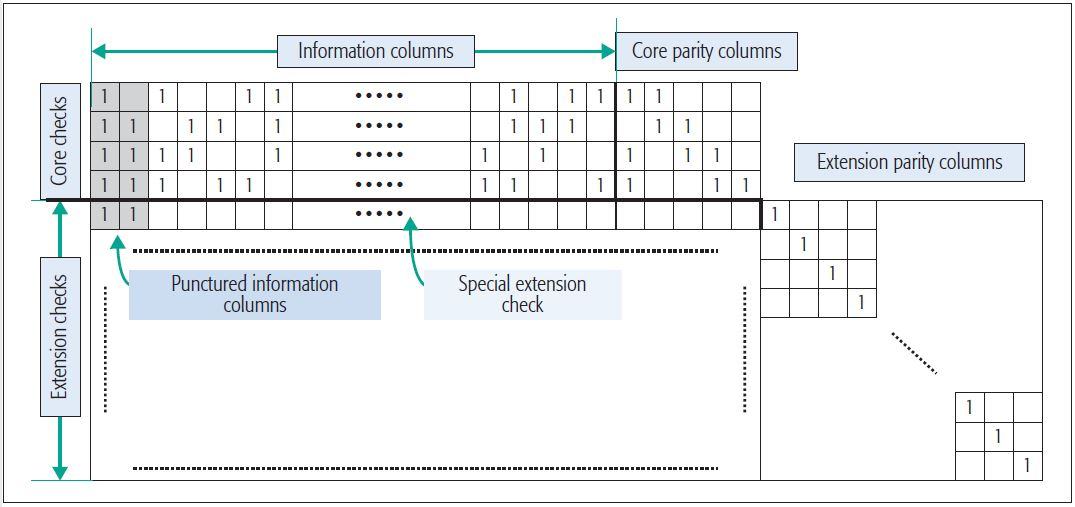
\includegraphics[scale=0.38]{pics/matriks5g}\end{tabular}
%\end{tabular}
%\caption{Sketch of base parity check structure for the 5G-NR LDPC codes \footnote{\tiny{T. Richardson and S. Kudekar, “Design of low-density parity check codes for 5G new radio,” IEEE Communications Magazine, vol. 56, no. 3, pp. 28–34, March 2018.}}.}
%\label{5gsketch}
%\end{figure}
%\end{columns}
\end{frame}

%=======================================================
%=======================================================
\section{The Downscaled Technique for DVB-T2 LDPC Codes}
%--------------------------
\begin{frame}{The Downscaled Technique for DVB-T2 LDPC Codes}
%--------------------------
\begin{columns}
\column{.5 \textwidth}
\begin{table}[tb]
\begin{adjustbox}{width=0.8\textwidth , totalheight=\textheight-2\baselineskip,keepaspectratio}
	\begin{tabular}{|l|l|l|lllll}
		\hline
		\multicolumn{1}{|c|}{20} & \multicolumn{1}{c|}{712}  & \multicolumn{1}{c|}{2386} & \multicolumn{1}{c|}{6354} & \multicolumn{1}{c|}{4061} & \multicolumn{1}{c|}{1062} & \multicolumn{1}{c|}{5045} & \multicolumn{1}{c|}{5158} \\ \hline
		\multicolumn{1}{|c|}{21} & \multicolumn{1}{c|}{2543} & \multicolumn{1}{c|}{5748} & \multicolumn{1}{c|}{4822} & \multicolumn{1}{c|}{2348} & \multicolumn{1}{c|}{3089} & \multicolumn{1}{c|}{6328} & \multicolumn{1}{c|}{5876} \\ \hline
		\multicolumn{1}{|c|}{22} & \multicolumn{1}{c|}{926}  & \multicolumn{1}{c|}{5701} & \multicolumn{1}{c|}{269}  & \multicolumn{1}{c|}{3693} & \multicolumn{1}{c|}{2438} & \multicolumn{1}{c|}{3190} & \multicolumn{1}{c|}{3507} \\ \hline
		\multicolumn{1}{|c|}{23} & \multicolumn{1}{c|}{2802} & \multicolumn{1}{c|}{4520} & \multicolumn{1}{c|}{3577} & \multicolumn{1}{c|}{5324} & \multicolumn{1}{c|}{1091} & \multicolumn{1}{c|}{4667} & \multicolumn{1}{c|}{4449} \\ \hline
		\multicolumn{1}{|c|}{24} & \multicolumn{1}{c|}{5140} & \multicolumn{1}{c|}{2003} & \multicolumn{1}{c|}{1263} & \multicolumn{1}{c|}{4742} & \multicolumn{1}{c|}{6497} & \multicolumn{1}{c|}{1185} & \multicolumn{1}{c|}{6202} \\ \hline
		0                        & 4046                      & 6934                      &                           &                           &                           &                           &                           \\ \cline{1-3}
		1                        & 2855                      & 66                        &                           &                           &                           &                           &                           \\ \cline{1-3}
		2                        & 6694                      & 212                       &                           &                           &                           &                           &                           \\ \cline{1-3}
		3                        & 3439                      & 1158                      &                           &                           &                           &                           &                           \\ \cline{1-3}
		4                        & 3850                      & 4422                      &                           &                           &                           &                           &                           \\ \cline{1-3}
		5                        & 5924                      & 290                       &                           &                           &                           &                           &                           \\ \cline{1-3}
		6                        & 1467                      & 4049                      &                           &                           &                           &                           &                           \\ \cline{1-3}
		7                        & 7820                      & 2242                      &                           &                           &                           &                           &                           \\ \cline{1-3}
		8                        & 4606                      & 3080                      &                           &                           &                           &                           &                           \\ \cline{1-3}
		9                        & 4633                      & 7877                      &                           &                           &                           &                           &                           \\ \cline{1-3}
		10                       & 3884                      & 6868                      &                           &                           &                           &                           &                           \\ \cline{1-3}
		11                       & 8935                      & 4996                      &                           &                           &                           &                           &                           \\ \cline{1-3}
		12                       & 3028                      & 764                       &                           &                           &                           &                           &                           \\ \cline{1-3}
		13                       & 5988                      & 1057                      &                           &                           &                           &                           &                           \\ \cline{1-3}
		14                       & 7411                      & 3450                      &                           &                           &                           &                           &                           \\ \cline{1-3}
	\end{tabular}
	            \end{adjustbox}

\end{table}
\column{.5 \textwidth}
\begin{itemize}

\item State the scaling factor $s_f$, where the factor must be divisors of $360$.  $360$ is the number of node indices of DVB-T2 LDPC codes.
\item Fill $p_{1}(j), p_{2}(j), p_{3}(j), \dots, p_{q}(j), j= 1, 2, 3, \dots, J$  and $q= 1, 2, 3, \dots, Q$. 
\item Calculate $r_{1}(j), r_{2}(j), r_{3}(j), \dots, r_{q}(j)$
		  \begin{eqnarray}
r_{q}(j) &=& mod \{ \left [ p_q(j) + j_{max}\times \left ( k-1 \right ) \right ], \nonumber \\  && \left [ P/s_f \right ] \} , \\ 1< k\leq \left ( 360/s_f \right )
		  \end{eqnarray}
\item The new table of addresses parity bit accumulators $r_q$ are obtained.

\end{itemize}
%Where $q$ is amount of column and $j$ is amount of row from addresses of parity bit accumulators, $s_f$ is the scaling factor, $P$ is amount of $N-K$ in the original DVB-T2 LDPC codes, and the range of k is $1< k\leq \left ( 360/s_f \right )$. 
\end{columns}
\blfootnote{\tiny{F. A. Newagy and S. H. Elramly, “Novel Technique for Scaling Down LDPC Code Lengths in DVB-T2 Standard,” in 2012 International Conference on Telecommunications and Multimedia (TEMU), July 2012, pp. 180–184.}}
\end{frame}

%--------------------------
\begin{frame}{The Downscaled Technique for DVB-T2 LDPC Codes (2)}
%--------------------------
\begin{figure}
\centering 
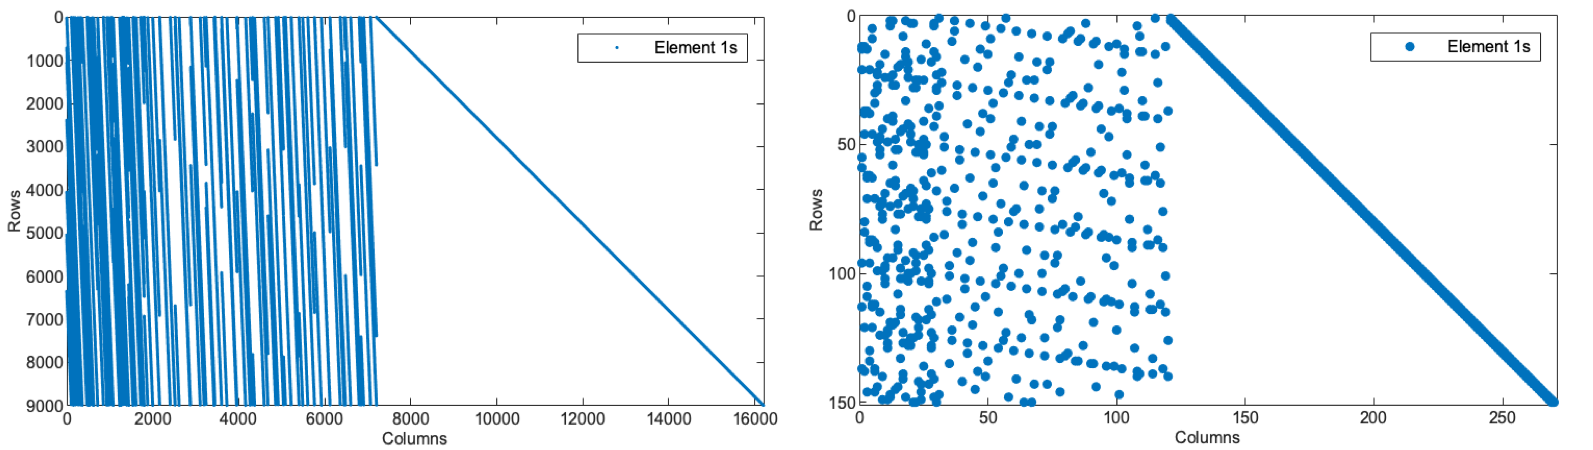
\includegraphics[scale=0.4]{gambarafa/compareH}
\caption{The comparison between parity check matrix of LDPC codes with a block length $N_{LDPC} = 16200$ and $N_{LDPC} = 270$.}
\label{sistemmodelMQCLDPC} %~\ref{kucing}
\end{figure}

By using $s_f=60$ the LDPC codes with block length $N_{LDPC}=16200$, so the size of matrix LDPC codes will be smaller become $N_{LDPC}=270$.



%\begin{table}[tb]
%		\caption{addresses of parity bit accumulators for $N_{LDPC}=16200$ with code rate $R=\frac{1}{2}$.}
%	\label{table:accu}
%	\begin{tabular}{|l|l|l|lllll}
%		\hline
%		\multicolumn{1}{|c|}{20} & \multicolumn{1}{c|}{712}  & \multicolumn{1}{c|}{2386} & \multicolumn{1}{c|}{6354} & \multicolumn{1}{c|}{4061} & \multicolumn{1}{c|}{1062} & \multicolumn{1}{c|}{5045} & \multicolumn{1}{c|}{5158} \\ \hline
%		\multicolumn{1}{|c|}{21} & \multicolumn{1}{c|}{2543} & \multicolumn{1}{c|}{5748} & \multicolumn{1}{c|}{4822} & \multicolumn{1}{c|}{2348} & \multicolumn{1}{c|}{3089} & \multicolumn{1}{c|}{6328} & \multicolumn{1}{c|}{5876} \\ \hline
%		\multicolumn{1}{|c|}{22} & \multicolumn{1}{c|}{926}  & \multicolumn{1}{c|}{5701} & \multicolumn{1}{c|}{269}  & \multicolumn{1}{c|}{3693} & \multicolumn{1}{c|}{2438} & \multicolumn{1}{c|}{3190} & \multicolumn{1}{c|}{3507} \\ \hline
%		\multicolumn{1}{|c|}{23} & \multicolumn{1}{c|}{2802} & \multicolumn{1}{c|}{4520} & \multicolumn{1}{c|}{3577} & \multicolumn{1}{c|}{5324} & \multicolumn{1}{c|}{1091} & \multicolumn{1}{c|}{4667} & \multicolumn{1}{c|}{4449} \\ \hline
%		\multicolumn{1}{|c|}{24} & \multicolumn{1}{c|}{5140} & \multicolumn{1}{c|}{2003} & \multicolumn{1}{c|}{1263} & \multicolumn{1}{c|}{4742} & \multicolumn{1}{c|}{6497} & \multicolumn{1}{c|}{1185} & \multicolumn{1}{c|}{6202} \\ \hline
%		0                        & 4046                      & 6934                      &                           &                           &                           &                           &                           \\ \cline{1-3}
%		1                        & 2855                      & 66                        &                           &                           &                           &                           &                           \\ \cline{1-3}
%		2                        & 6694                      & 212                       &                           &                           &                           &                           &                           \\ \cline{1-3}
%		3                        & 3439                      & 1158                      &                           &                           &                           &                           &                           \\ \cline{1-3}
%		4                        & 3850                      & 4422                      &                           &                           &                           &                           &                           \\ \cline{1-3}
%		5                        & 5924                      & 290                       &                           &                           &                           &                           &                           \\ \cline{1-3}
%		6                        & 1467                      & 4049                      &                           &                           &                           &                           &                           \\ \cline{1-3}
%		7                        & 7820                      & 2242                      &                           &                           &                           &                           &                           \\ \cline{1-3}
%		8                        & 4606                      & 3080                      &                           &                           &                           &                           &                           \\ \cline{1-3}
%		9                        & 4633                      & 7877                      &                           &                           &                           &                           &                           \\ \cline{1-3}
%		10                       & 3884                      & 6868                      &                           &                           &                           &                           &                           \\ \cline{1-3}
%		11                       & 8935                      & 4996                      &                           &                           &                           &                           &                           \\ \cline{1-3}
%		12                       & 3028                      & 764                       &                           &                           &                           &                           &                           \\ \cline{1-3}
%		13                       & 5988                      & 1057                      &                           &                           &                           &                           &                           \\ \cline{1-3}
%		14                       & 7411                      & 3450                      &                           &                           &                           &                           &                           \\ \cline{1-3}
%	\end{tabular}
%\end{table}

\end{frame}


%=======================================================
%=======================================================

%%--------------------------
%\begin{frame}{Encoding of LDPC Codes}
%%--------------------------
%\begin{columns}
%\column{.45\textwidth}
%\begin{figure}
%\centering
%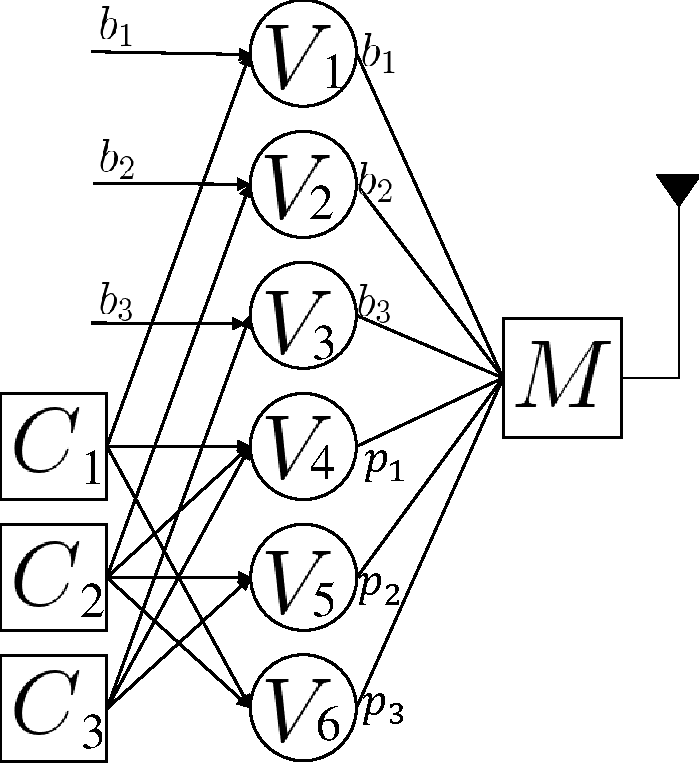
\includegraphics[scale=0.4]{pics/encoder2.pdf}
%\caption{Example for Tanner graph of Generator matrix LDPC codes.}
%\end{figure}
%
%\column{.55\textwidth}
%Information bits $b=\{b_1, b_2, ..., b_k\}$ are generated randomly, where $k$ is the number of bits in one block code.
%Generator Matrix $\mathbf{G}$ shows CND $ \mathbf{C} $, \textit{interleaver} $\Pi_x$, and VND $ \mathbf{V} $ in transmitter. The encoded codeword $\mathbf{c}$ can be written as
%\begin{equation}
% \mathbf{c}=\mathbf{b\:G}.
% \label{eqc}
%\end{equation}
%$c(k)$ is mapped to the complex modulation $M$ based on
%\begin{eqnarray}
%x(k)=\frac{1}{\sqrt{2}}[(1-2c(k))+j(1-2c(k))].
%\end{eqnarray}
%
%\end{columns}
%\end{frame}


%--------------------------
\begin{frame}{The Proposed Downscaled DVB-T2 LDPC Codes (1): Degree Distribution}
%-------------------------- 

{\footnotesize  $R=\frac{4}{9}$ 
\begin{eqnarray}
\lambda (x)&=&\frac{1}{270}x+\frac{149}{270}x^2+\frac{90}{270}x^3+\frac{30}{270}x^8 \\
\rho(x)&=&\frac{25}{150}x^4+\frac{53}{150}x^5+\frac{60}{150}x^6+\frac{12}{150}x^{12},
\end{eqnarray}
$R=\frac{2}{3}$ 
\begin{eqnarray}
\lambda (x)&=&\frac{1}{270}x+\frac{89}{270}x^{2}+\frac{162}{270}x^{3}+\frac{18}{270}x^{13},\\
\rho(x)&=&\frac{1}{90}x^{9}+\frac{89}{90}x^{10},
\end{eqnarray}
$R=\frac{3}{5}$
\begin{eqnarray}
\lambda (x)&=&\frac{1}{270}x+\frac{107}{270}x^2+\frac{132}{270}x^3+\frac{30}{270}x^{12},\\
\rho(x)&=&\frac{1}{108}x^8+\frac{107}{108}x^9,
\end{eqnarray}
}
\end{frame}
%=======================================================
%=======================================================
\begin{frame}{The Proposed Downscaled DVB-T2 LDPC Codes (2): Degree Distribution}
$R=\frac{11}{15}$
\begin{eqnarray}
\lambda (x)&=&\frac{1}{270}x+\frac{71}{270}x^{2}+\frac{192}{270}x^{3}+\frac{6}{270}x^{12},\\
\rho(x)&=&\frac{7}{48}x^{15}+\frac{17}{48}x^{16}+\frac{18}{48}x^{17}+\frac{6}{48}x^{18},
\end{eqnarray}
$R=\frac{7}{9}$
\begin{eqnarray}
\lambda (x)&=&\frac{1}{270}x+\frac{71}{270}x^2+\frac{198}{270}x^3,\\
\rho(x)&=&\frac{7}{60}x^{11}+\frac{29}{60}x^{12}+\frac{24}{60}x^{13},
\end{eqnarray}
$R=\frac{37}{45}$
\begin{eqnarray}
\lambda (x)&=&\frac{1}{270}x+\frac{71}{270}x^{2}+\frac{192}{270}x^{3}+\frac{6}{270}x^{12},\\
\rho(x)&=&\frac{7}{72}x^{9}+\frac{11}{72}x^{10}+\frac{36}{72}x^{11}+\frac{12}{72}x^{12} \nonumber \\ &&+\frac{6}{72}x^{13}.
\end{eqnarray}


\end{frame}

%\begin{frame}{Extrinsic Information Transfer (EXIT) Chart}
%\begin{columns}
%\column{0.7\textwidth}
%\begin{itemize}
%%\item Tujuan digunakan EXIT \textit{chart} pada jaringan super padat adalah mendesain jaringan \textit{Internet-of-Things} (IoT) di suatu kota. 
%\item EXIT chart use mutual information $I=1-v$ where $v$ is erasure probability $v=\{p,q\}$.
%\item Parameter $p$ and $q$ is erasure probability for CND and VND.
%\item EXIT chart shows extrinsic mutual information from VND
%\begin{eqnarray}
%I_{E,VND}(x)&=&1-\lambda(p) \nonumber\\
% &=&1-\lambda(1-I_{A,VND}), 
%\end{eqnarray}
%and extrinsic mutual information from CND
%\begin{eqnarray}
%I_{E,CND}(x)&=&\omega(1-q) \nonumber\\
% &=&\omega(I_{A,CND}).
%\end{eqnarray}
%\end{itemize}
%\column{0.35\textwidth}
%\begin{figure}
%	\centering
%	\includegraphics[width=0.8\textwidth]
%		{pics/erasure.pdf}
%		\caption{Edge probability from CND and VND}
%\end{figure}
%\end{columns}
%\end{frame}
     

%============================================================================
%==========================================================================
\section{Performance Evaluations}
%\begin{frame}
%\tableofcontents[currentsection,currentsubsection]
%\end{frame}
%--------------------------
%\begin{frame}{Performance Evaluation (1): EXIT Analysis}
%%--------------------------
%\begin{columns}
%\column{.5\textwidth}
%\vspace{-30pt}
%%\begin{figure}
%%\centering 
%%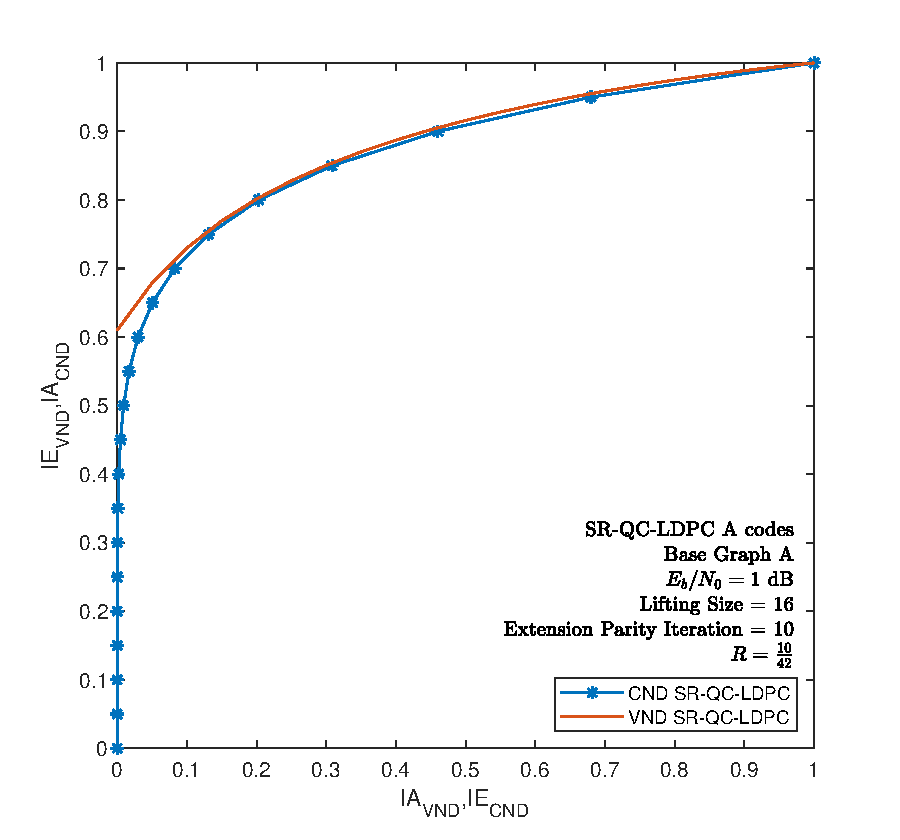
\includegraphics[scale=0.4]{pics/EXIT_QC_1.pdf}
%%\caption{EXIT chart of the proposed SR-QC-LDPC-A codes.}
%%\label{coba1} %~\ref{kucing}
%%\end{figure}
%
%\column{.5\textwidth}
%\vspace{-30pt}
%%\begin{figure}
%%\centering 
%%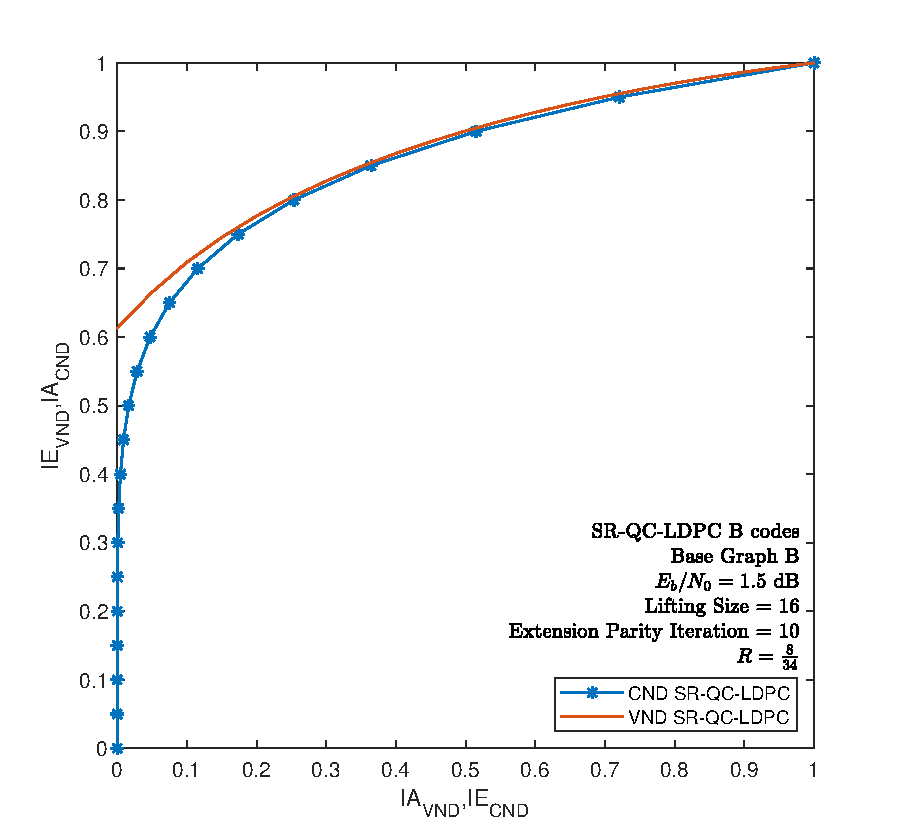
\includegraphics[scale=0.4]{pics/EXIT_QC_3.pdf}
%%\caption{EXIT chart of the proposed SR-QC-LDPC-B codes.}
%%\label{coba2} %~\ref{kucing}
%%\end{figure}
%\end{columns}
%EXIT curve of VND and CND shows that gap is minimal expressing that the loss of the proposed SR-QC-LDPC codes is minimal.
%\end{frame}

%--------------------------
\begin{frame}{Performance Comparison on AWGN Channel}
%--------------------------
\vspace{-25pt}
\begin{columns}
\column{.5\textwidth}
\begin{figure}
\centering 
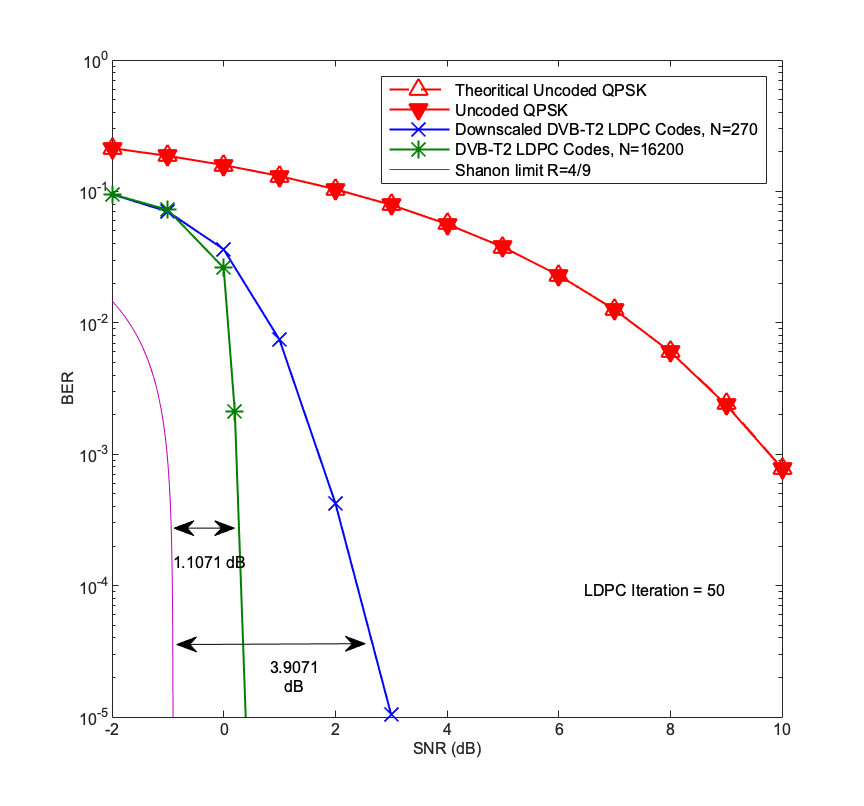
\includegraphics[scale=0.4]{gambarafa/AWGN}
\caption{BER performances of DVB-T2 LDPC codes with $R=\frac{4}{9}$ under AWGN channel.}
\label{awgn} %~\ref{kucing}
\end{figure}
\column{.5\textwidth}
\begin{itemize}
\item Gap between the Shannon limits for $R=4/9$ and  DVB-T2 LDPC codes with $N_{LDPC}=270$ is about $3.9~dB$ while the gap of DVB-T2 LDPC codes with $N_{LDPC}=16200$ is obtained about $1.1~dB$.
%\item The proposed SR-QC-LDPC codes is comparable with 5G NR QC-LDPC codes, where the obtained gap is about 0.75--1~dB.
\end{itemize}
\end{columns}
\end{frame}

%--------------------------
\begin{frame}{Performance Evaluation on Bandung Channel Models}
%--------------------------
\begin{columns}

\column{.45\textwidth}
\vspace{-25pt}
\begin{figure}
\centering 
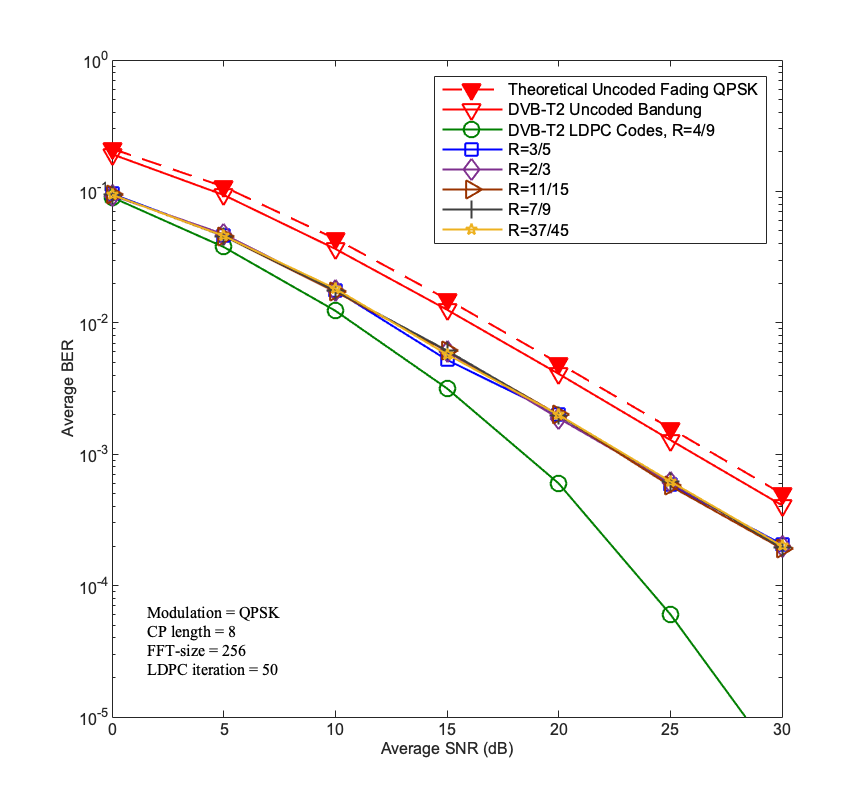
\includegraphics[scale=0.4]{gambarafa/coded-2}
\caption{BER performances Downscaled DVB-T2 LDPC codes codes under Bandung Channel models.}
\label{fading} %~\ref{kucing}
\end{figure}
\column{.55\textwidth}
\begin{itemize}

\justifying
\item The BER Performances of DVB-T2 LDPC codes with $R~=~\left \{ \frac{4}{9}, \frac{3}{5}, \frac{2}{3},\frac{11}{15},\frac{7}{9},\frac{37}{45} \right \}$ are evaluate under Bandung Channel models\footnotemark[1].
\item The best performances of Downscaled LDPC codes DVB-T2 on is achieved $10^{-4}$ at $R=\frac{4}{9}.$

\end{itemize}
\end{columns}
\blfootnote{\tiny{D. Fitriyani, K. Anwar, and D. M. Saputri, "Study on Radio Frequency Profile of Indonesia Digital Television DVB-T2 for Urban Areas", in 2019.}}

\end{frame}


%==============================================================================
%==============================================================================




%============================================================================
%==========================================================================

\section{Conclusion}
%\begin{frame}
%\tableofcontents[currentsection,currentsubsection]
%\end{frame}
\begin{frame}{Conclusion}
%--------------------------
\begin{itemize}
\justifying
\item This paper has provided the BER performances comparison between DVB-T2 LDPC codes with block length $N_{LDPC}=16200$ and downscaled DVB-T2 LDPC codes with $N_{LDPC}=270$. 
\item This paper provide the BER performances of downscaled DVB-T2 LDPC codes in all rate at Bandung Channel Model.
\item The gap between DVB-T2 LDPC codes  $N_{LDPC}=16200$ and downscaled DVB-T2 LDPC codes $N_{LDPC}=270$ is about $2.8~dB$
\item The best code rate of downscaled DVB-T2 LDPC codes under Bandung Channel model is $R=\frac{4}{9}$.
\item The results are expected to be one of the solutions for implementation of DVB-T2 in Indonesia. 
%\item The performances of rateless capability have also been confirmed to be better than that of the fixed rate under the fading channels. 
%\item The codes are expected to be useful for further development of dynamic channel changes.
\end{itemize}
\end{frame}



%--------------------------
%\begin{frame}{Conclusion}
%%--------------------------
%\begin{itemize}
%\justifying
%\item This paper has proposed SR-QC-LDPC codes inspired from the Raptor encoding principle of 5G NR QC-LDPC codes. 
%\item The SR-QC-LDPC codes have been designed by reducing the matrix size and removing the high degree, of which the final designs are evaluated using EXIT chart. 
%\item We found that the codes have excellent EXIT curve matching where small gap is kept although the size of the matrix is reduced. 
%\item The performances of rateless capability have also been confirmed to be better than that of the fixed rate under the fading channels. 
%\item The codes are expected to be useful for further development of dynamic channel changes.
%\end{itemize}
%\end{frame}

%==============================================================================
%==============================================================================

\end{document}
